%\documentclass[12pt,a4paper]{article}
%\usepackage[ngerman]{babel}

\documentclass[12pt,a4paper,final]{article}
\usepackage[T1]{fontenc}
\usepackage[utf8]{inputenc}
\usepackage[ngerman]{babel}
\usepackage{amsmath}
\usepackage{amsfonts}
\usepackage{amssymb}
\usepackage{lmodern}
\usepackage[left=2cm,right=2cm,top=2cm,bottom=2cm]{geometry}
\usepackage{graphicx}
\usepackage{hyperref}
\usepackage{listings}
\usepackage{fancyvrb}
\title{BCDWristWatch}
\date{\vspace{-10ex}}
\begin{document}
\pagenumbering{gobble}
\title{BCDWristWatch}
\author{SulKith}
\maketitle
\vspace{5cm}
\begin{center}
  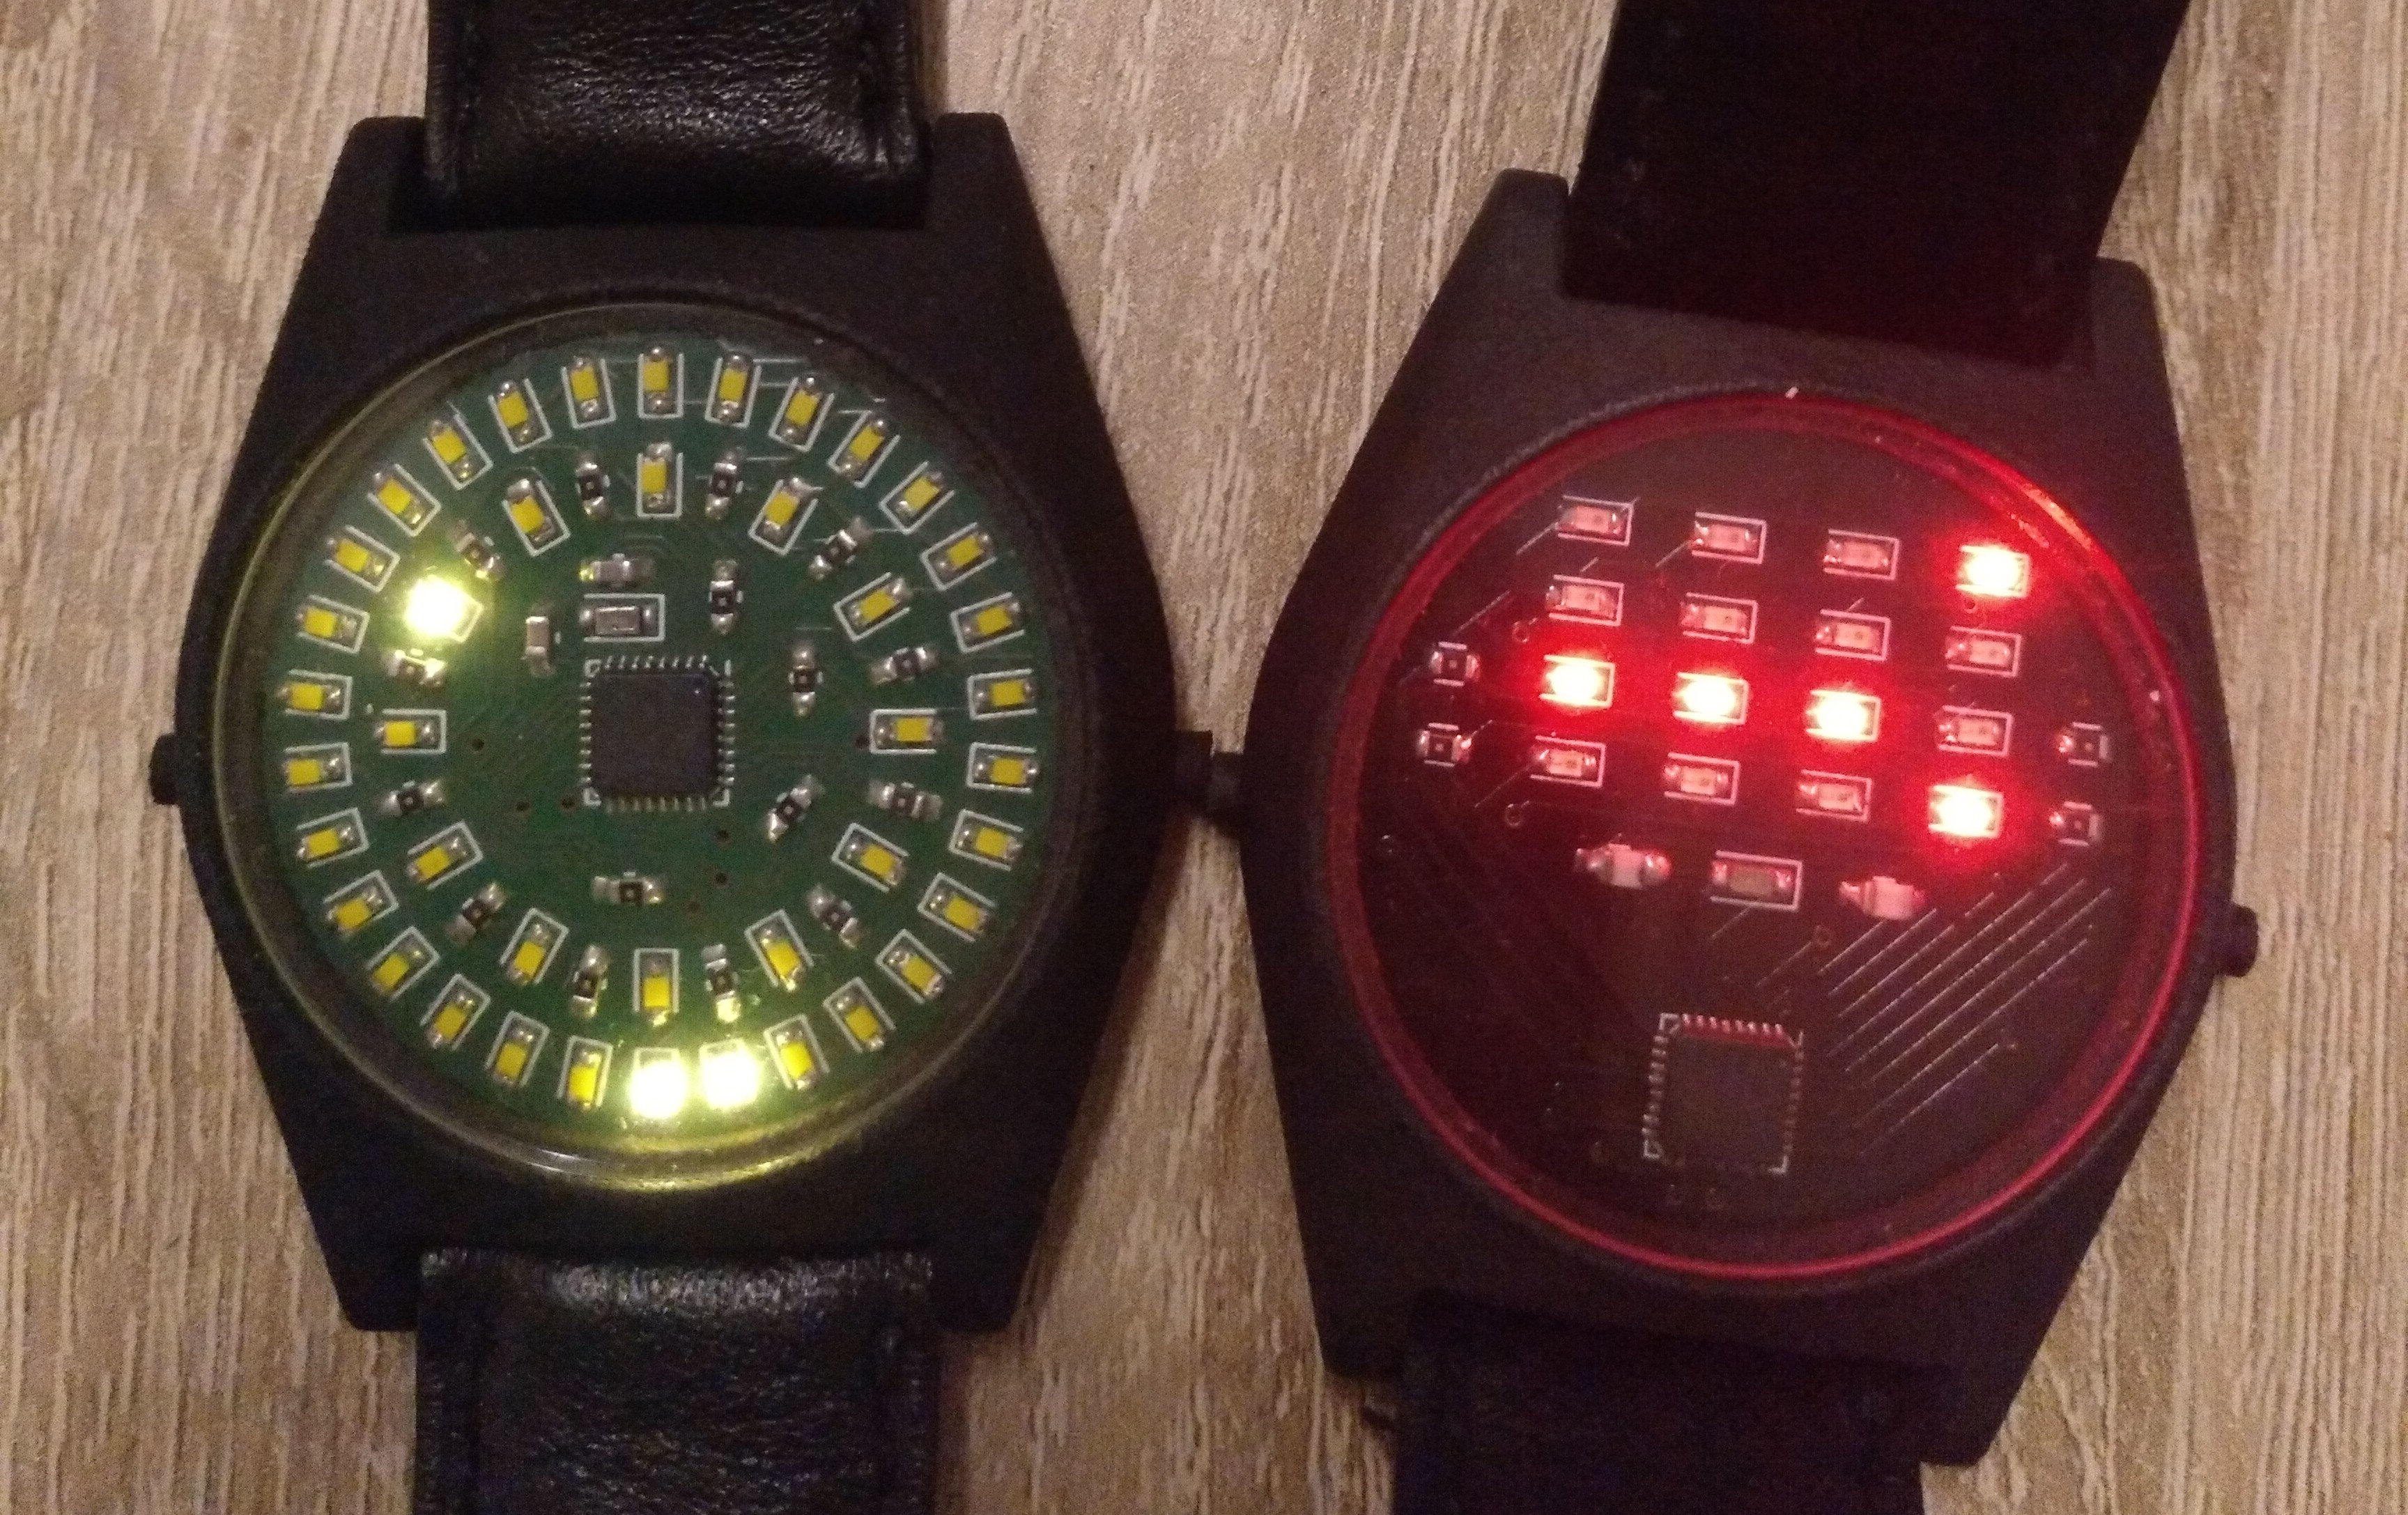
\includegraphics[width=\textwidth]{../Pictures/AnalogClock.jpg}
\end{center}
\newpage
\section*{Summary}
It all started with the idea of a PCB which could display the time in BCD code and is small enough to wear it on the wrist. Sadly i was not able to find a Housing which could be used for the Clock, so i created one myself in OpenSCAD and 3D-printed it.
After a while i got tired to explain the BCD code to everybody, so there is also a Analogish Version available.

The Software for both Versions is unified and just differentiated by the Linker. So there is no change to the Code needed.

After some problems with sweat entering the Housing and destroying the electronics, i tried several possible solutions (read more in the story).
\\
\\
The alternative try to solve the sweat issue was to remove the buttons completely and replace them with a G-Force sensor. As sensor the Bosch BMA456 is used, since it features various interrupt functionalities to wakeup the microcontroller and only draws a few microamps in standby.

The powerful Sensor also made some other cool features for a wrist watch.
There is a Wrist Tilt detection to activate the Watchface once the user rises the arm and takes a look on the watch. Now the watch can also be turned on while only using one hand e.g. while carrying stuff.

Another cool new feature is a stepcounter, so the watch is also a (not completely sweat resistant ;-) ) fitness tracker.

The next evolution step is switching to a new more powerful controller. For this the STM32L432K Controller was chosen. This controller also features a calender in the built in RTC.
\newpage
\section{Binary Watch}
\subsection{PCB}
\subsubsection{First PCB Version}
The First PCB Version was a desaster. The PCBs arrived very fast, but the QFN Package had the wrong size.
ATMEL only produces QFN32 in 7x7mm. Therefore the design of the PCB hat to be changed to the smaller package,
but that gave me the Chance to shrink the Design to a smaller form factor.
The part which keeps the PCB from getting smaller is the Coin Cell Battery (CR2032).
On the PCBs there was the order number printed on the Front side, which would be visble in the final assembly.
\subsubsection{Second PCB Version}

The second PCB Version was designed from scratch. But the Front was the side with the Battery, so hopefully the Order Number would not be printed on the visible side of the PCB. This worked out very well for the second Version of the PCBs.
\subsubsection{PCB1}

since the PCBs finally arrived. it was possible to assemble all the parts.
The first PCB was assembled with some Cables soldered to the Testpins on the Backside of the Board.
And the Battery case was also not assembled.
Here is a Picture of the uncleaned but already soldered PCB
\begin{center}
  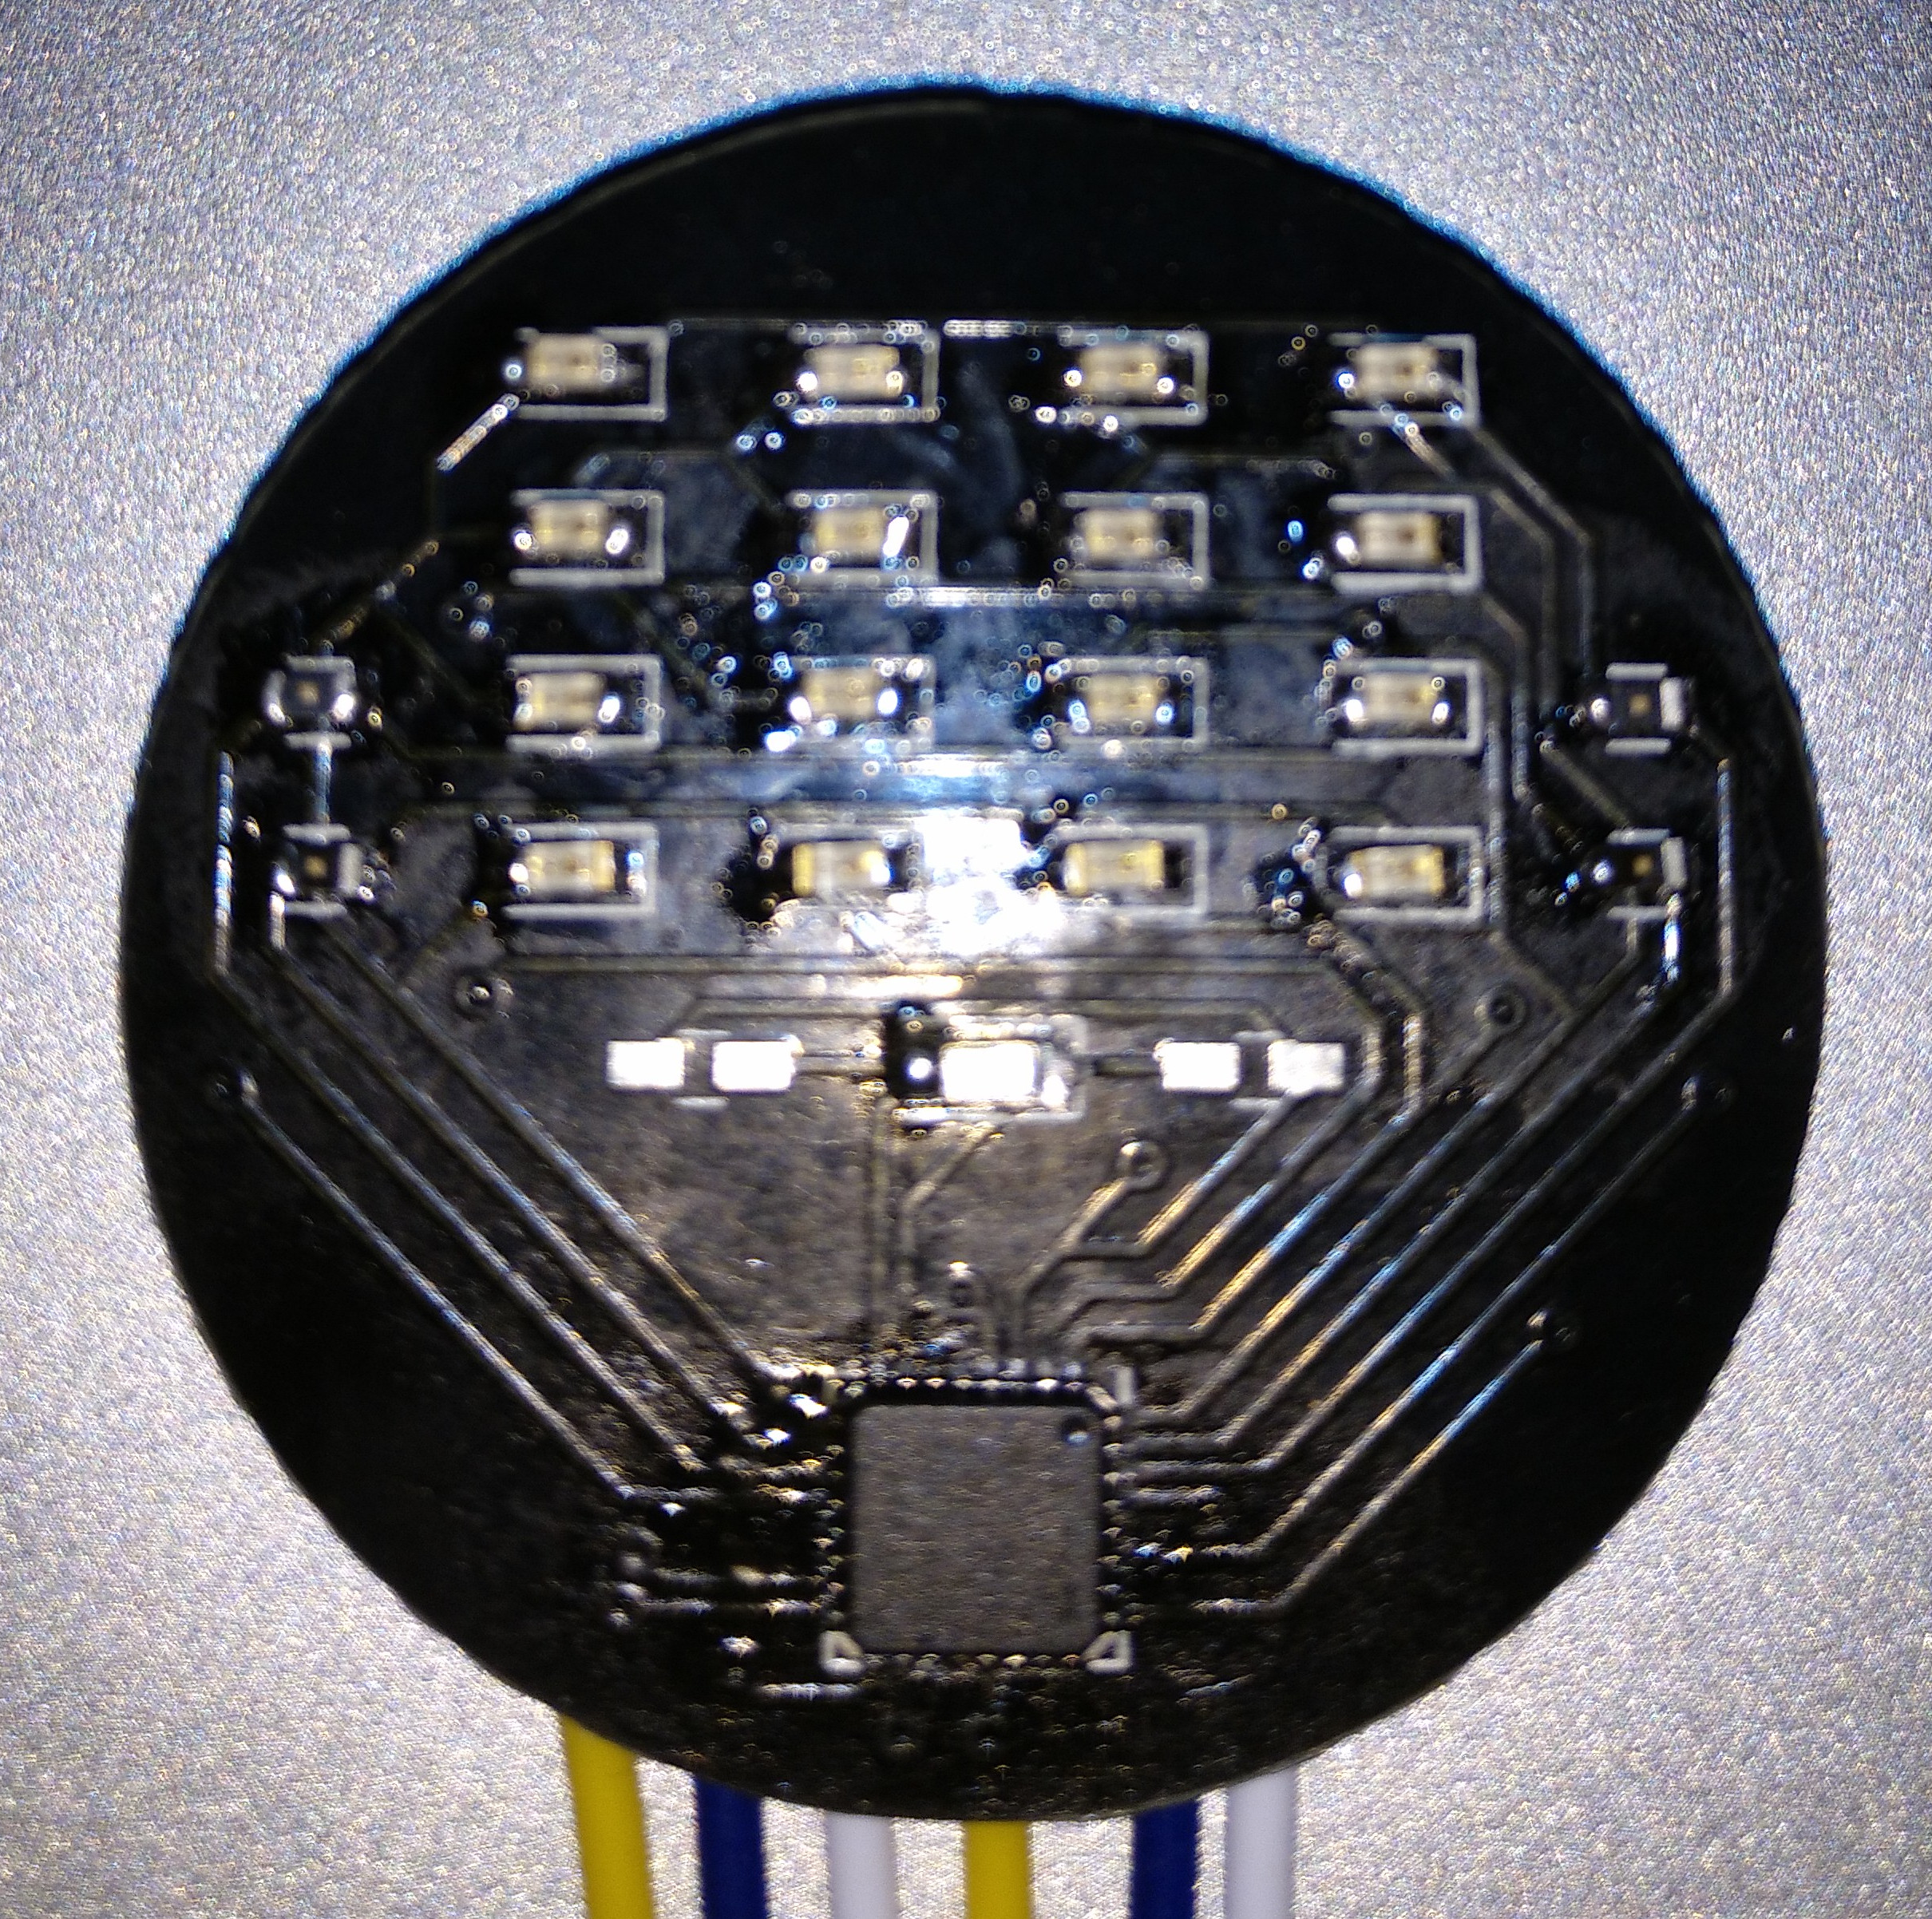
\includegraphics[width=0.5\textwidth]{../Pictures/PCB1_F1.jpg}
\end{center}

\subsubsection{PCB2}
The PCB2 was assembled and cleaned as a First Prototype with the Housing.\
Here aretwo Pictures of the PCB one without the LEDs turned on and one with the LEDs turned on.\
Brightness was set in the Program to 100/255 (see software void showLEDs, constant perc=100) 
\begin{center}
\includegraphics[width=0.45\textwidth]{../Pictures/PCB2_F1_off.jpg} \includegraphics[width=0.45\textwidth]{../Pictures/PCB2_F1_on.jpg}

\end{center}

\subsubsection{PCB3}
The third PCB was ordered at \href{https://aisler.net}{aisler.net}. It only took around one and a half week to arrive(to Germany).\
The PCB was not completely milled out. It was in a carrier PCB with rectangular shape, but it was easy to remove.\
I had to sand the edges a bit, since it was a bit rough on the parts where i removed the connections to the carrier, since i had to sand the PCB anyway to fit in the Housing that was no big problem.\
The overall Quality of the PCBs is very good, but you can not choose the thicknes or color of the PCB.\
\begin{center}
  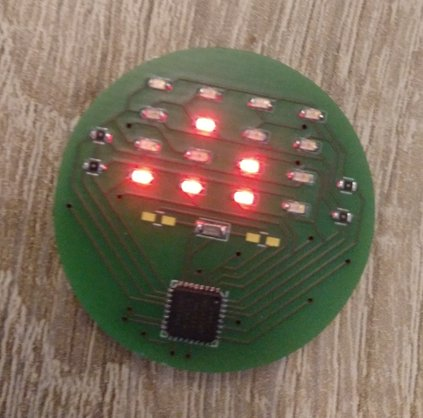
\includegraphics[width=0.5\textwidth]{../Pictures/PCB3.jpg}
\end{center}

\newpage

\subsection{Housing}
The Housing was designed in OpenSCAD.\
a very helpfull reference for the OpenSCAD syntax was\
\url{https://en.wikibooks.org/wiki/OpenSCAD_User_Manual/Transformations}

\subsubsection{Housing 1}
The Housing was printed by the TOOM Printing Service as SLS in PLA.\
Sadly all the surfaces are not really smooth, therefore the Buttons are working very bad.\
I tried to glue in the glass with superglue, but the glue dried out white, this looks really bad :-(\

\subsubsection{Plans for Housing 2}
The next housing should be produced via SLA with transparent Resin, so no glass for Protection is needed, 
since the resin could be used.
\paragraph{Problems while printing with SLA}
It turns out, that there is no completely transparent Resin available. All of them get a yellow color sooner or later.
So it is not really beautiful as a glass.

\subsubsection{Housing 2}
A friend told me that most of the time the resin will not reflect light equally in every spot, therefore i decided to order a PCB without glass and do the mounting of the glass with very tight tolerances and a rim on the top edge.\
this worked out extremely well.\
Another goal was to make the second Housing slim, because the first one was very bulky. With a bit of optimization is was possible to integrate the bottom plate completely in the housing. The overall thicknes was reduced from about 15mm to 9.4mm with the 1mm PCB or 10mm with the new 1.6mm PCB.\
For the PCB to tightly fit in either the Housing has to get some aditional holes or at least the Battery clip has to be modified.\
\begin{center}
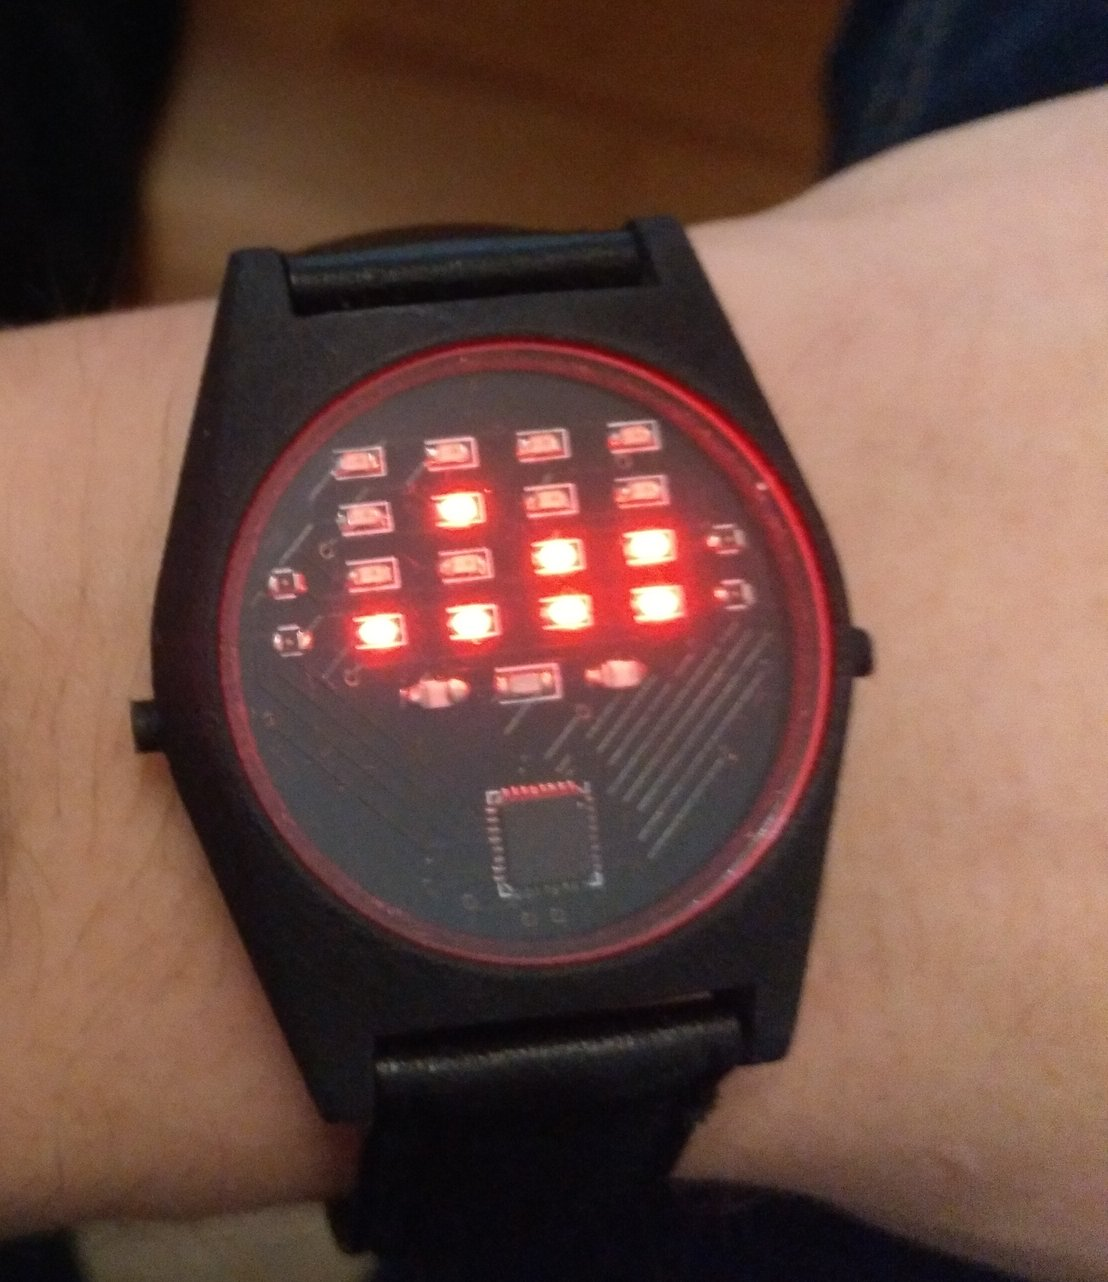
\includegraphics[width=0.45\textwidth]{../Pictures/Housing2.jpg} 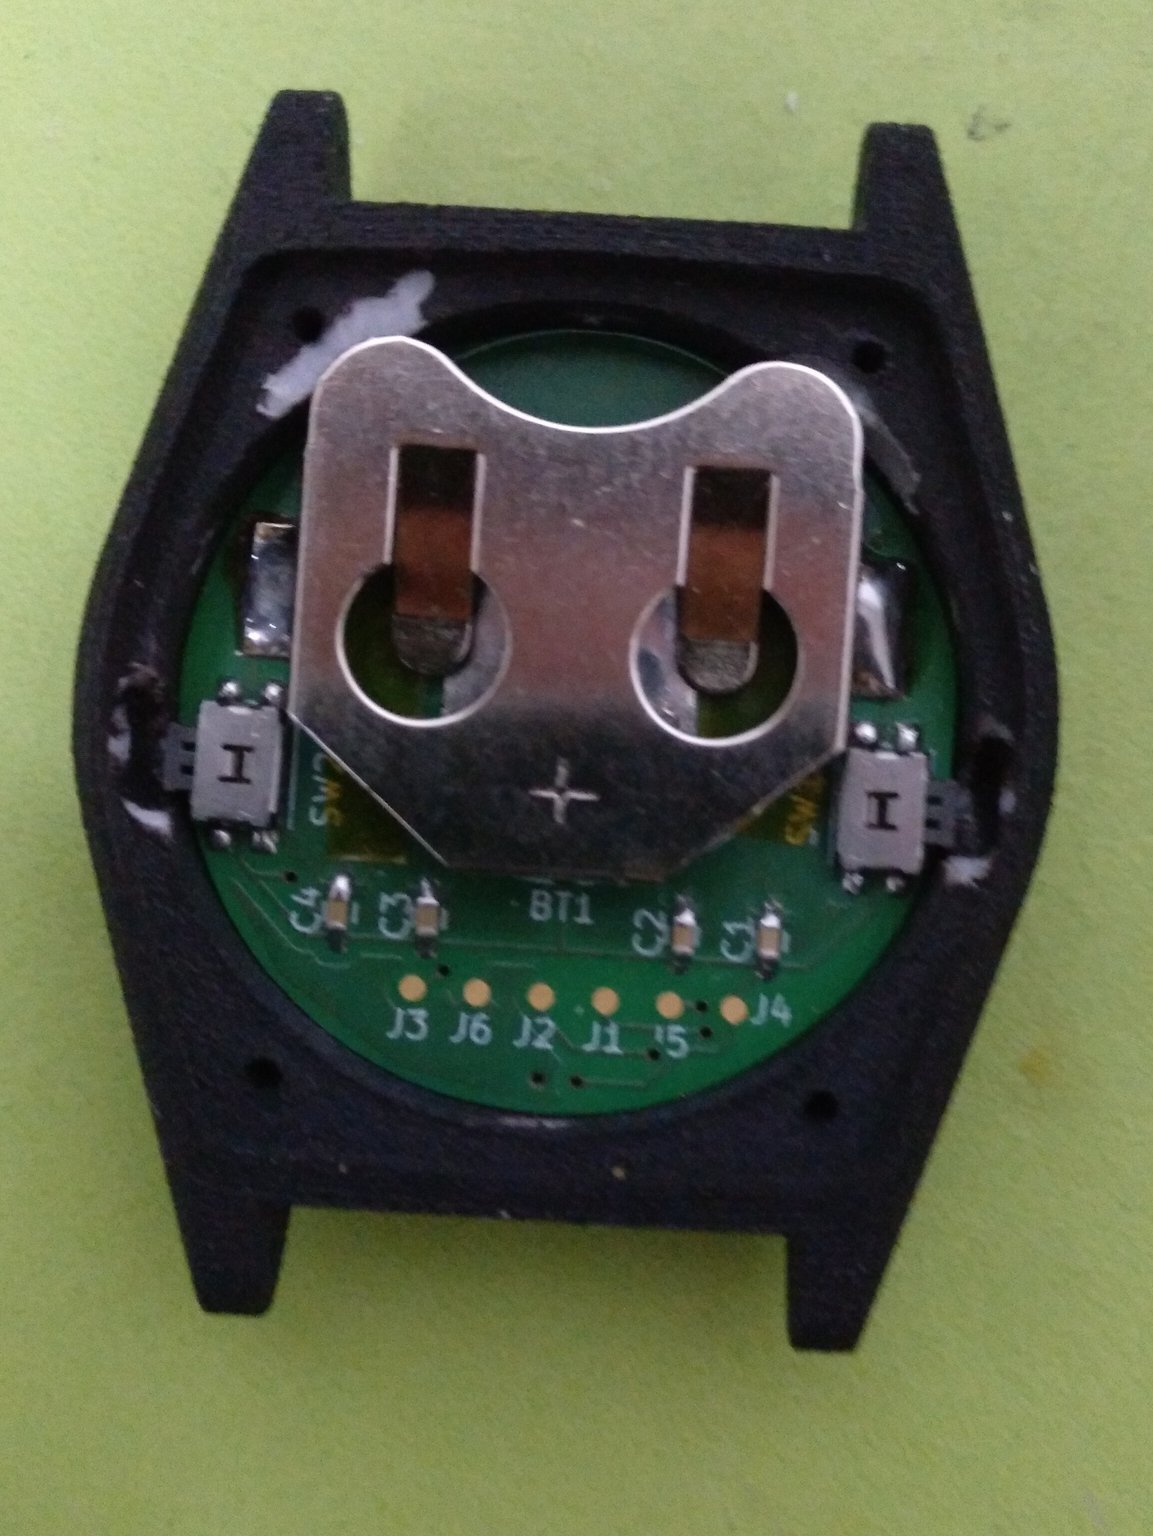
\includegraphics[width=0.45\textwidth]{../Pictures/Housing3b.jpg}
\end{center}

\subsection{Problems}
\subsubsection{Sweat is entering the Housing}
The first watch broke down after nearly 1 year. After opening the Housing the Problem was very obvious. Sweat was entering the Housing and corroded the PCB and the mounted parts.
\begin{center}
  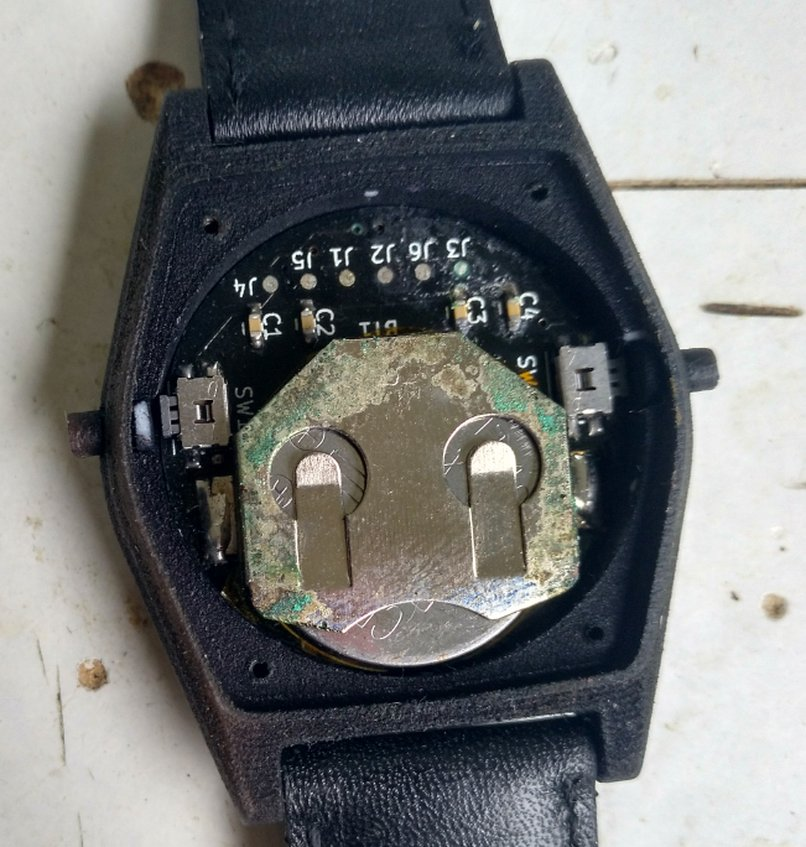
\includegraphics[width=0.5\textwidth]{../Pictures/ProbCorr1.jpg}
\end{center}
\paragraph{Cleaning the PCB and adding something to absorb the moisture}
As a solution i tried to clean the PCB with Isopropanol and glued some rice to the PCB to absorb the moisture, that helped only for about a week and the Watch stopped working again. So that is not the best solution, but is is an extraordinary try ;-)
\begin{center}
  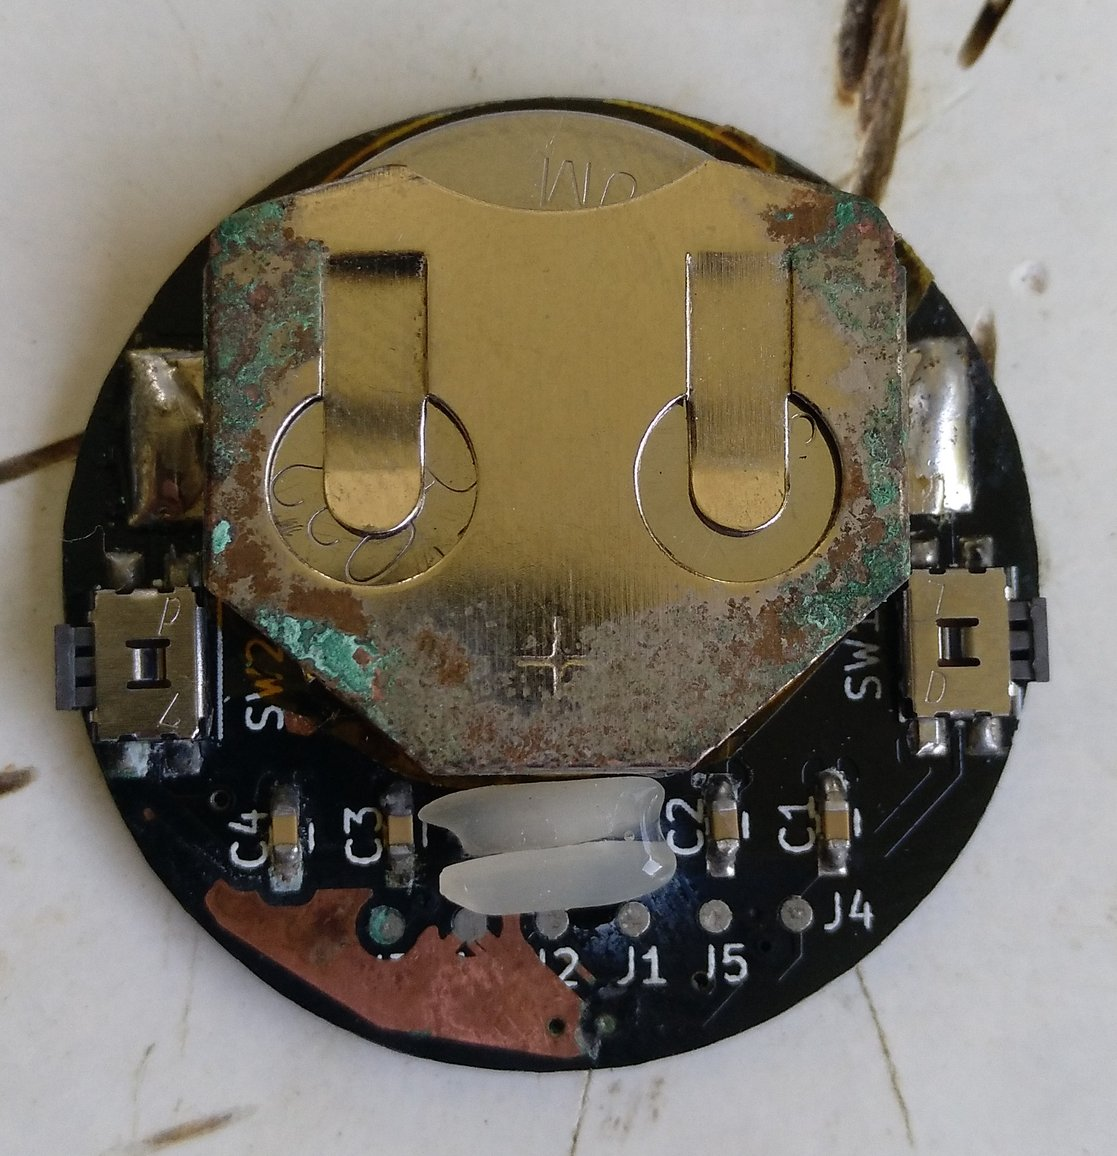
\includegraphics[width=0.5\textwidth]{../Pictures/ProbCorrSol1.jpg}
\end{center}
\paragraph{adding isolation Tape between the lid and the housing}
The second solution was to add Tape, which is originally designed to be used to seal threads, between the housing and the lid.\
That worked out a little bit better, but the Watch also stopped working after a few weeks. 
\paragraph{Analyzing the Watch again}
After analyzing it again the PCB seemd to be ok. The PCB was only a little damaged from the first sweat attack.
The Problem was that the time stopped to run, but another point was that the LEDs wont go off anymore. 
But it was possible to set the time. 
So the conclusion is that the clock which is run by the crystal stopped running.
\paragraph{Adding clear Nailpolish to guard the Crystal}
The next attempted solution was to add clear Nailpolish to the PCB, so the crystal is completely covered. This is an attempt to stop moisture from crawling below the crystal and stopping the clock.

Adding Nailpolish was also not the real solution. The Clock also stopped to work after a few weeks.

\paragraph{commercial products to insulate PCBs}
The next attempt will be to use a commercial Product to insulate the PCB.
For this i will try \href{https://www.reichelt.de/korrosionsschutzlack-plastik-70-super-400-ml-isolierlack-kontakt-32046-p125737.html}{Plastik 70 Super} from Kontakchemie.
\subsection{Manual}
\subsubsection{How to read the Watch}
The time is displayed in BCD Code. For further reference please see the Picture below:
\begin{center}
  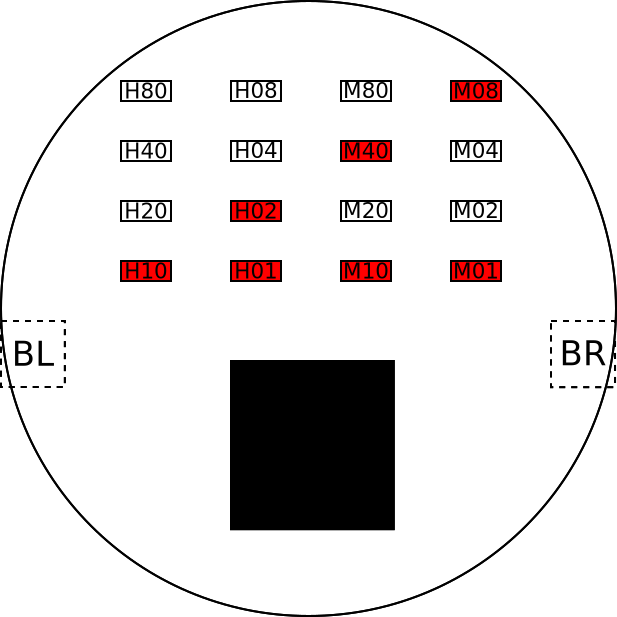
\includegraphics[width=0.5\textwidth]{drawings/BinDia1359.png}
\label{fig:BinWatchFace}
\end{center}
There are Two Buttons on the Watch:
\begin{itemize}
	\item BL: left Button
	\item BR: right Button
\end{itemize}
To read the Watch it is necessary to activate the Display via one of the Buttons

The LEDs are read columnwise. So the right two columns are showing the Minutes. If an LED is litone have to add its Value to the Minutes if not then nothing is added. So for the full hour no led in the right two columns will be lit.

In the Example above the following LEDs are lit: M40, M10, M08 and M01.
The sum of all the values is the current minute value $40+10+8+1=59$

The Hours are displayed exactly like the Minutes. For the hours the 24 Hour Format is used. In the Example above the following LEDs are lit: H10, H01, H02. The current Hour Value is also determined by summing everythin up: $10+1+2=13$.

So the current Time in the example is 13:59. If it is 0:00 the watch will display 24:00 to make sure 0:00 is not confused with a broken watch.
\subsubsection{set the time}
To set the time first of all the display has to be activated, afterwards both buttons have to be released (to make sure that the setup mode is not accessed accidently). Now both buttons have to be pressed. Now the LED H80 lights up, to signalize that now it is in set hour mode. Now Both buttons can be released again.

To switch to the set minute mode the right button has to be pressed. In set minute mode the right button switches back to the normal mode.

With the right button the value which is set currently can be incremented.
The hour will not be incremented wen incrementing the minutes from 59 to 0.

Both setup modes will timeout if no button is pressed for 30 seconds.
While the watch is in setup mode the clock will be stopped, after returning to normal mode the seconds will start from 0 so it is easy to set the time precisely.


\newpage
\section{Analog Watch}
\subsection{PCB}
After the PCBs for the BCD Version were working, i also created an analog Version, so i dont have to explain the Clock everytime ;-)

The Analog Watch features the same Schematics for the basic clock functionality, but the display is done via Charlieplexing the LEDs. There are 4 Clustes with 4 Pins which drive all the 42 LEDs. 12 LEDs on the inner ring are displaying the hours. On the outer ring 30 LEDs display the Minutes. Since it was not possible to fit 60 LEDs on the outer ring, uneven numbers are shown while lighting up the two neighbouring LEDs.
\begin{center}
  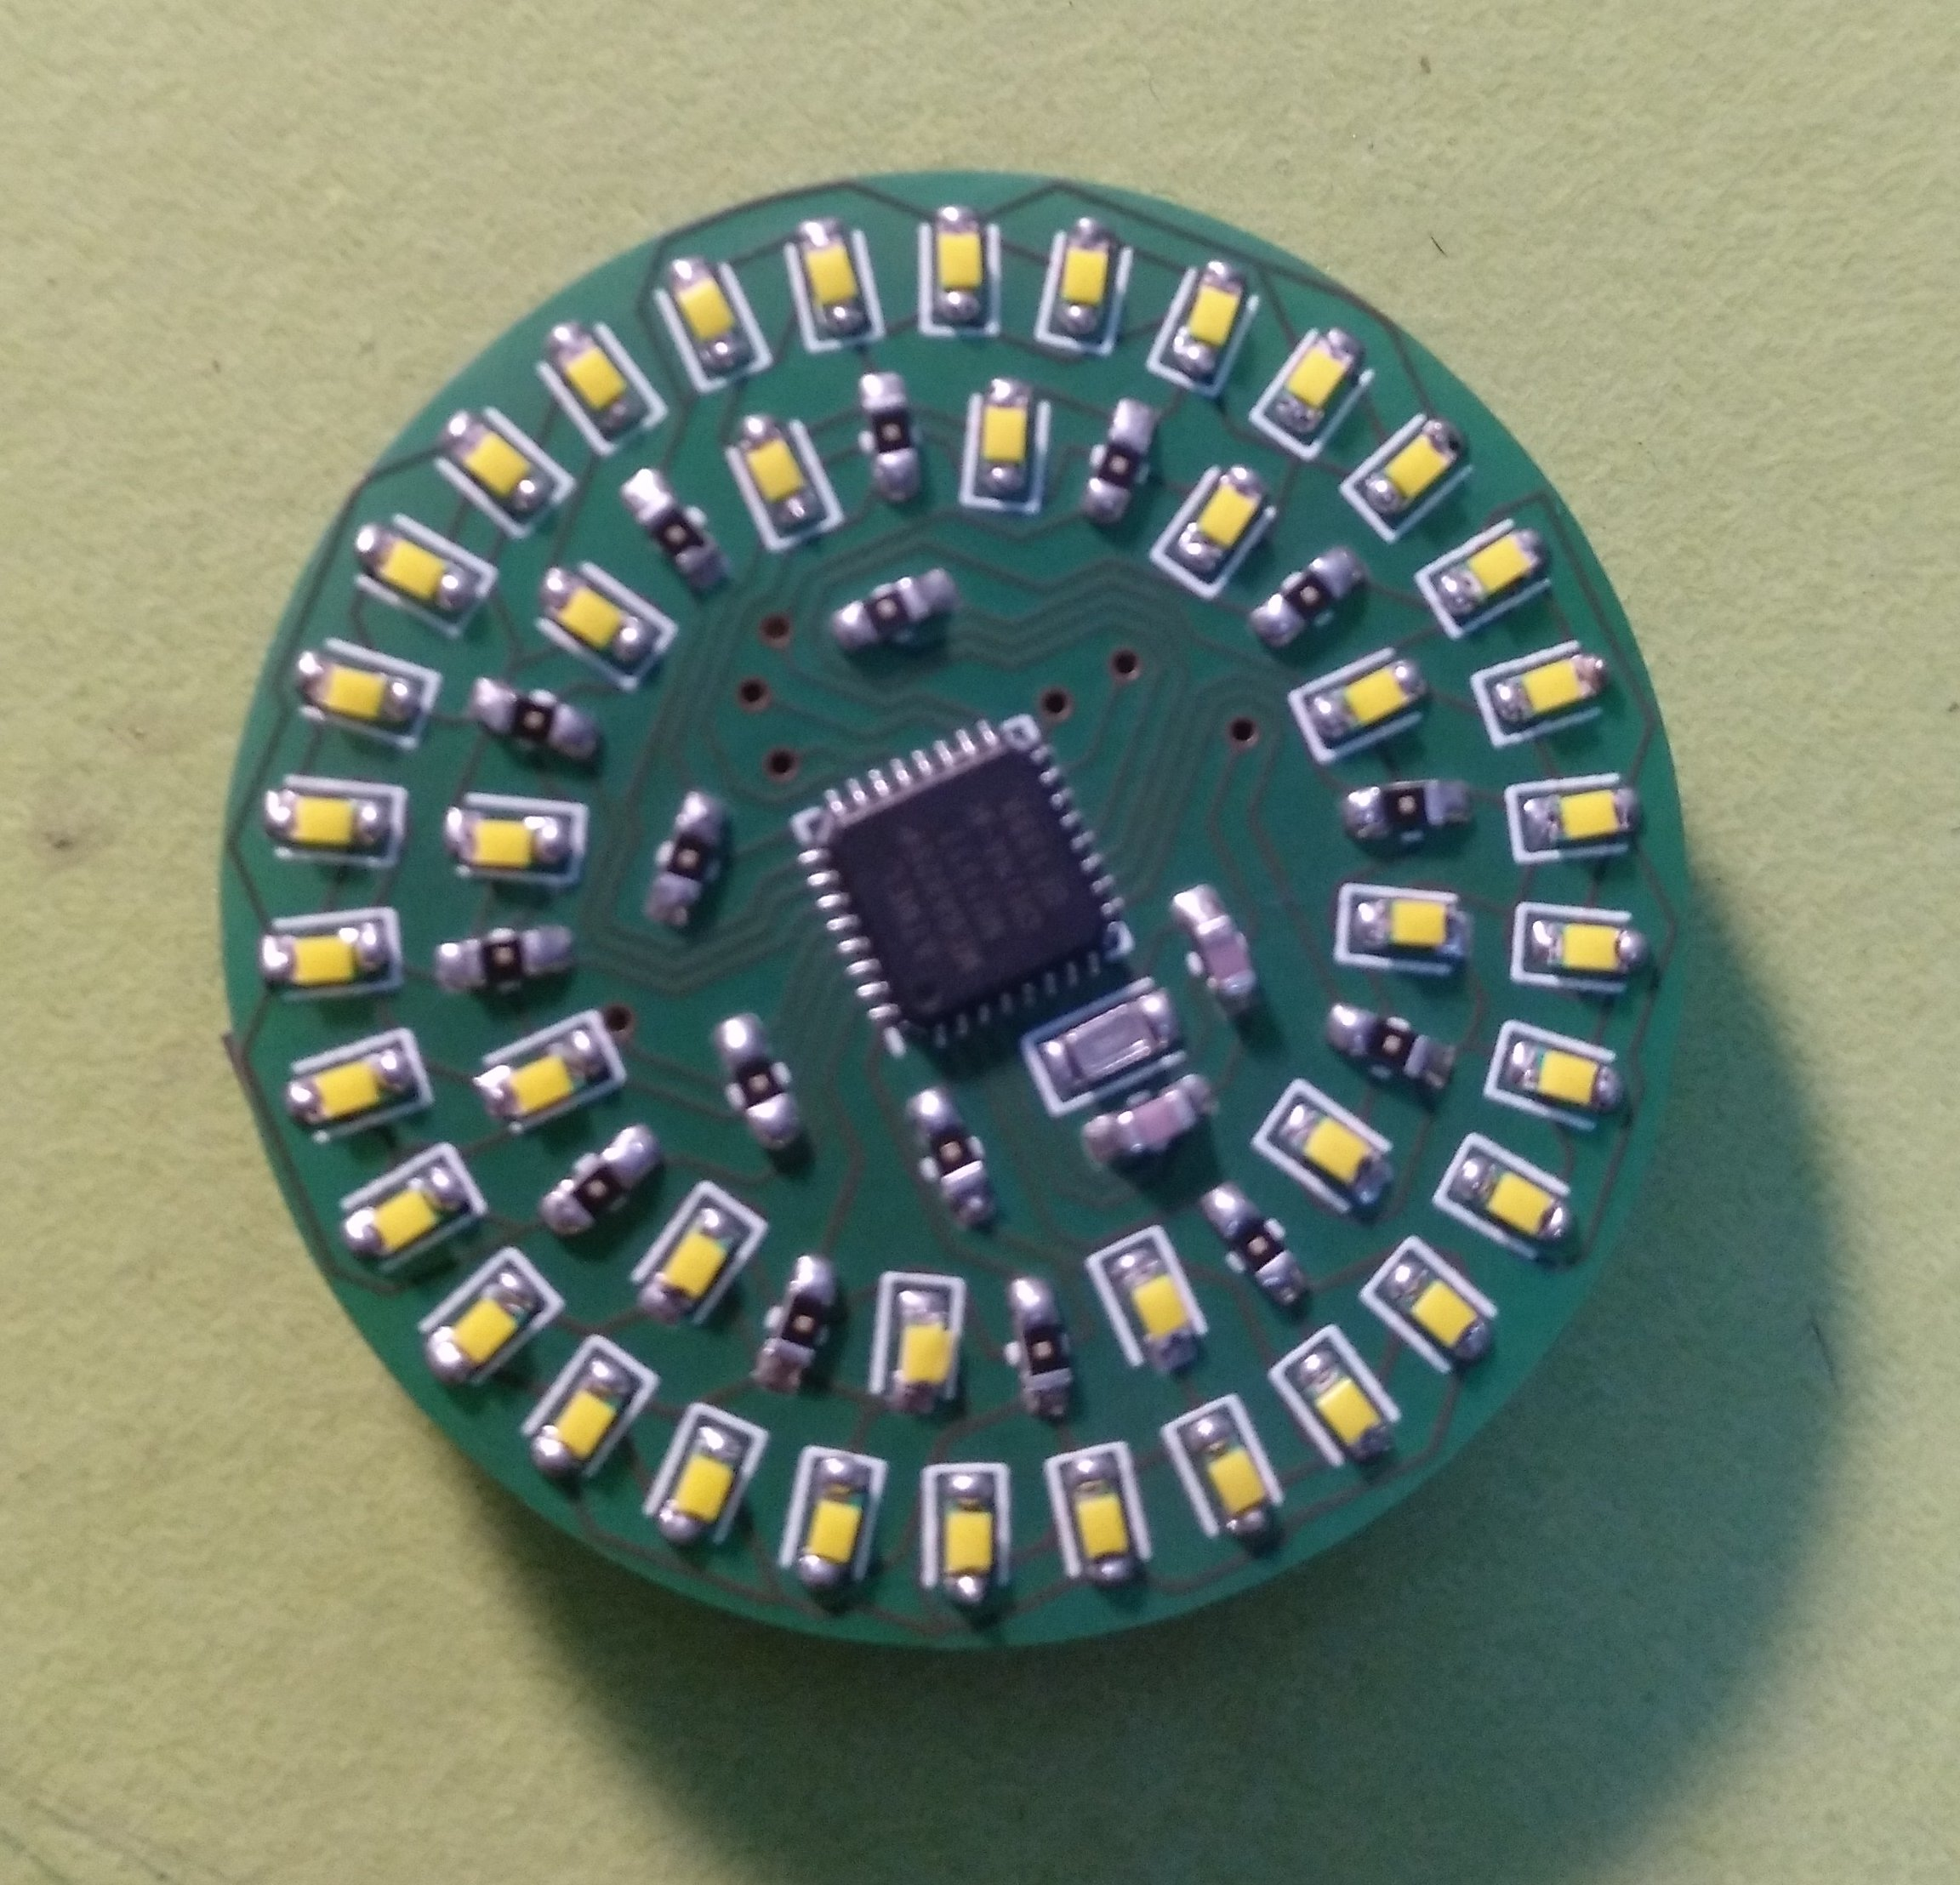
\includegraphics[width=0.5\textwidth]{../Pictures/AnalogPCB.jpg}
\end{center}
\newpage

\subsection{Housing}
The PCB for the analog Version is designed with the same mechanical Interface as the Binary Version therefore the Housing from the Binary Version can be used.

\subsection{first Watch which i gave away}
The first Watch i gave away was one of the analog PCB ones i built for my dads birthday.
for this Watch i replaced all the resistors for the LEDs with Zero $\Omega$ resistors, so the LEDs got more bright and are clearly readable also in the sunlight.
\begin{center}
  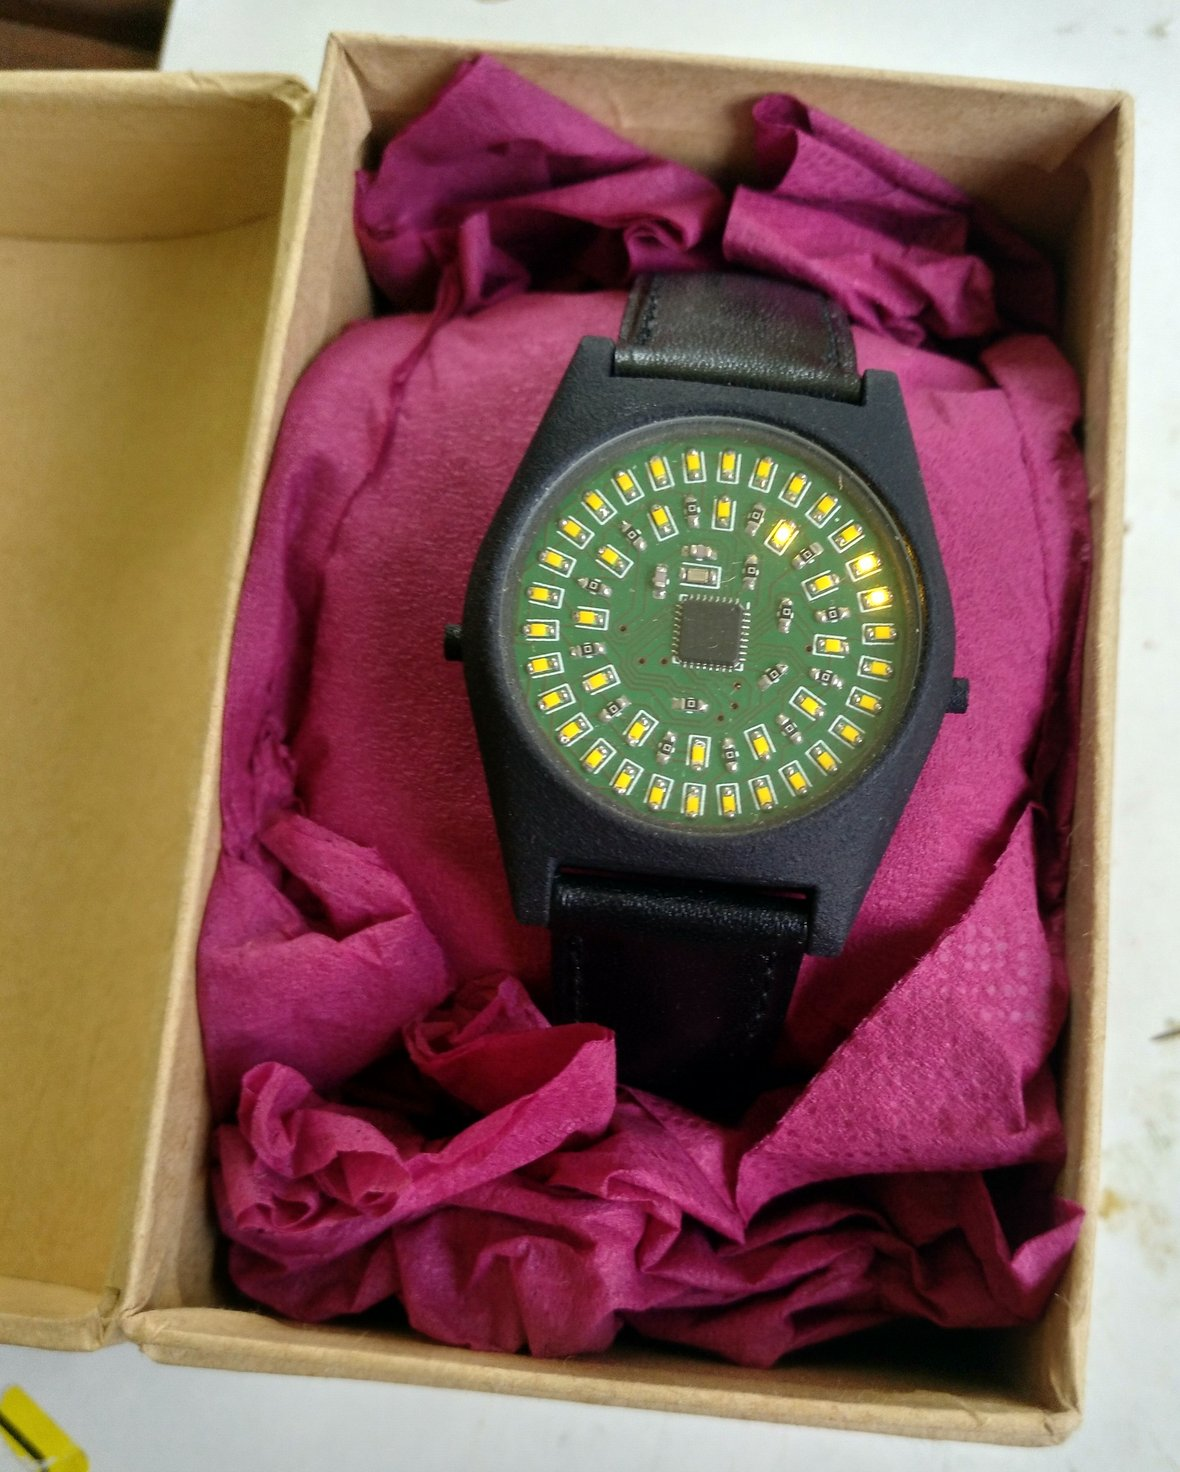
\includegraphics[width=0.7\textwidth]{../Pictures/AnalogWatch1.jpg}
\end{center}
\section{BinaryGWatch}
\subsection{PCB}
The PCB is based on the Binary Watch. Even the Buttons would still work if soldered on the board. Additionally to the original Schematics there is a Bosch BMA456 connected to the SPI, which is already on the back of the PCB to enable programming via Pogo Pins. Additionally there is also the Chip select pin used and two interrupt pins to enable the wakeup functionality via the BMA sensor

The BMA Sensor is mounted on the back of the PCB to keep the symetric watch face. 

The concept is to use the BMA Sensor also as interface. To enable the Display and also to set the time. So no buttons will be needed this should also enable a housing without holes to keep sweat from crawling into and solve the corroded PCB problems I had with the first BinaryWatch
\section{Switching to an ARM Controller}
The obvious next evolution step would be to include the BMA Sensor into the analog Version. But since the ATMega328P has a lot of reserved pins there are not enough usable pins to supply the BMA and the 42 LEDs (only one Pin was missing). So there were a few possible solutions
\subsection{AVR Controller in a bigger Package}
Regarding the Software this would be the easiest Varaint to go with.
But there are a few disadvantages of the AVR Controller.
\begin{itemize}
	\item a larger Package requires more PCB Space
	\item it requires 6 Pins for ISP programming
	\item it has a bigger power consumption than modern Controllers
	\item modern Controllers are faster
	\item it is an old Controller ;-)
	\item there is no technical challenge 
\end{itemize}
So this was not the final solution.
\subsection{Atmel SAM}
I started with the Atmel SAM Controller, because I liked the experience with Atmel Controllers so far. For a comparison of Microcontrollers there is a great article from Jay Carlson \url{https://jaycarlson.net/microcontrollers/}. The advantage of the Atmel SAM Controllers are there are a lot of open source Tools which could also be used out of a makefile, so the projectsrtucture is very easy to create. All the Configuration and the Bootupsequence is generated by the Atmel Start utility. \url{https://start.atmel.com/}. The feature i liked the most is the SERCOM Interface.A SERCOM interface could be used for various serial Interfaces (UART, I2C, SPI...), the biggest advantage is that all thepins could be multiplexed with each other.

Therefore i created a Evaluationboard i could start playing around with:
\url{https://github.com/sulkith/devboards/tree/master/ATSAML22G18A_LowPowerArm}

Once the Board arived i encountered the first problem. The files generated by the Atmel Start utility are licensed under the ASF license. And since i'm no lawyer, i couldn't really decide if it is safe to use these files in an open-source project like this one. So i decided to build a wrapper, which would unpack the Package generated by the Atmel Start utility and include the files in my project Structure (\url{https://github.com/sulkith/devboards/blob/master/ATSAML22G18A_LowPowerArm/Software/AtmelStart/AtmelStartIntegrate/importAtzip.sh}). But as soon as you need to change some code in the Startup or in the drivers the whole process is not working anymore.

But since in the early stages one has to change a lot of settings in the configurator and include it back in my code. So the whole Workflow is some kind of clumpsy. And i got a bit sick of changing a Setting and taking one or two minutes to change a single option. So i was looking for a solution where the whole process is smoother.

\subsection{STM32}
So a few colleques suggested to go for a STM32 Controller because the STMCubeIDE is very smooth and all configurations are done inside the IDE.Afterwards the Code is directly generated. A big plus point was that in the copiright notice it is explicitely stated, that you are allowed to redistribute the software if you mention the original source(this is automatically done in the header of every file). So using it for an open source project doesn't seem to be a problem.

\subsubsection{STM32L053R8}
To start with the ecosystem i went for a Nucleo-L053R8 development board with a lowpower Cortex M0+. It took me about half an hour to get the I2C running. So the IDE is great and easy to use. The Controller used on the Board is featuring a on-chip RTC which is also running in all Low-Power modes including Standby mode. So all the Timekeeping wor the wrist watch could be done completely by the chip. There is also a RTC-Clibration feature, which could be used to syncronize the deviation of the Crystal with a high precision frequency source. 
Sadly the STM32L053R8 Controller is not available in a QFN32 Package.

\subsubsection{STM32L432K} 
While searching for a replacement for the STM32L053R8 i came across the STM32L432K Controller, with a Cortex M4 Core, which is also featuring a Shutdown mode with only about 400 nA with the RTC running. So the Watch will consume very low power. A Wakeup is also possible by the Wakeup pin, which could be connected to the BMA Controller to wake up the Controller on wrist tilt or double-tap. There are enough pins for using the Wakeup Pin, SPI, SWD-Debugging and supplying all 42 LED for the analog version.
So from the Hardware point of view everything is fine.

\paragraph{Binary PCB}
Sinc the ST QFN Package looks like a big black box i also placed the BMA456 sensor, which also looks like a black box right next to it for a more PCB like look.
\begin{center}
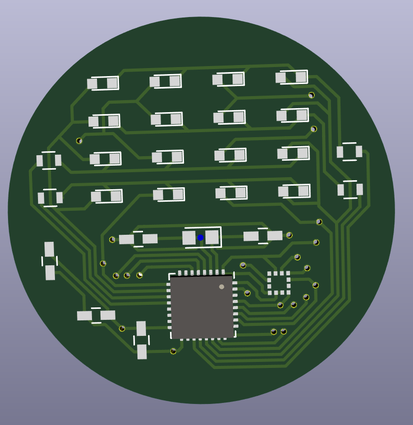
\includegraphics[width=0.45\textwidth]{../Schematics/Schematics_STM/Watch.png}
\end{center}
\paragraph{The Boot Pin}
When the first PCBs arrived it was very easy to get them working, but when the Debugger was not connected sometimes the controller wasn't booting correctly and was displaying strage things on the LED. When connecting to the controller without a reset one could identify the courrent all stack. And the address was in the section of the ST Bootloader. So the obvious suspect was the Boot Pin, the pin was floating in the initial PCB design and this is a bad Idea. In the first Prototype this was fixed by connecting it directly to the neighbouring ground pin. For the next version there will be a resistor pulling it to ground.

Since the Watch was working now it was time to get the crystal calibration working. But since the controller only has a 32 Pin Package the Calibration Pin is not available in the footprint. 

\paragraph{Calibration}
A Workaround for the missing calibration feature was to use the Timer in frequency counter mode with the LSE clock(External Crystal) connected to the Clock pin. So the Input timervalue will be saved on each Signal edge, after two edges the difference could be calculated. For an input Frequency of 1Hz the difference has to be exactly 32768. To increase the accuracy was the presacaler was set to the maximum value of 8. So the value has to be exactly 8*32768. To further increase the accuracy the whole process will be repeated 20 Times and then the average deviation will be calculated. From this deviation the correction value per 1 ppm could be calculated. But after the calibration procedure the Watch was still not very acurate.

\paragraph{Load Capacitance}
While searching for the source of the Clock Deviattion i came across the Application Note 2867
\url{https://www.st.com/resource/en/application_note/cd00221665-oscillator-design-guide-for-stm8af-al-s-stm32-mcus-and-mpus-stmicroelectronics.pdf} Which describes the Design guidelines for oscillators used in combination with STM32 controllers. The crystal used in the Clock is the Abracon ABS05W-32.768 kHz-D. The AN2867 recommends 4pF Load Capacitors for this setup. Till now i used 10pF Capacitors, this could als explain the heavy correction which was needed for the AtMega328P.

So i did a few single measurements to measure the difference of the Changes done. The measurements were done with the same Controller on the same PCB, once with a Battery Supply (2.8V) and once with Power Supply from the Nucleo Board (3,3V), The second change was the Change of the Capacitors from 10pF to 3,9pF (i couldn't get exactly 4pF on the 0603 Package). The Results could be found in the Table below.
\vspace{1cm}

\begin{tabular}{|l|l|l|l|}
\hline
Supply Voltage {[}V{]} & Load Capacitance {[}pF{]} & Frequency {[}Hz{]} & Deviation {[}ppm{]} \\ \hline
2,8   & 10                        & 32549              & -209                \\ \cline{2-4} 
                       & 3,9                       & 32850              & 92                  \\ \hline
3,3   & 10                        & 32548              & -210                \\ \cline{2-4} 
                       & 3,9                       & 32857              & 99                  \\ \hline
\end{tabular}
\vspace{1cm}

So we can conclude that a larger Capacitance slows the oscillator down. The correction needed for the clock was now smaller, but the deviation was still there.

\paragraph{CubeIDE Initialization}
After another few tests i found out there is a relation between Wakeups and the Deviation of the Clock. So the original Proble was every time the Controller is initialized the code generated by the CubeIDE will initialize the whole Clock System. To initialize the driver strength of the LSE Clock the clock has to be stopped, and syncronized again. This Process will delay the RTC Time by about 0,5 seconds.

Therefore i needed to adapt the initialization for the Controller. The function, which was causing the Problems is the \verb!SystemClock_Config()!, if there is a LSE configured it would be initialized. So the obvoius solution would be to disable the LSE. But if the LSE is disabled the RTC would need a Clock, so the RTC was also disabled. The big Problem is if the RTC is disabled in the configuration the HAL Driver would not be included in the project. So i copied the initialization Function from the code generated without the RTC and renamed it to \verb!SystemClock_Config_without_LSE()! in the Project configuration i disabled the function call to the original \verb!SystemClock_Config()! and called the \verb!SystemClock_Config_without_LSE()! in the usermain instead. Also the RTC initialization had to be rewritten to only initialize the RTC if the LSE is not running. For this task the Function \verb!STM32L4_HAL::HAL_driverInit()! was introduced. This Function checks if a RTC clock source is set. The clock source is set in the \verb!RCC_BDCR! register, which resides in the backupdomain of the STM and therefore is not cleared by a reset. So the initialization will be only done once when the Battery is inserted.

\paragraph{Analog PCB}
Since the STM32L432K has more usable pins than the Atmega328P it was also possible to route a PCB with the BMA Sensor and the Analog Watchface.
The space for the Analog Watchface was already very tight without the BMA Sensor. With the Sensor it got extremely tight, so i had to turn the Controller by 45 Degrees. Sadly I was not able to comply with all the Designrules for the BMA Sensor. Now i have a via under the BMA, i think this is very bad for series production, but for me it is working.

\begin{center}
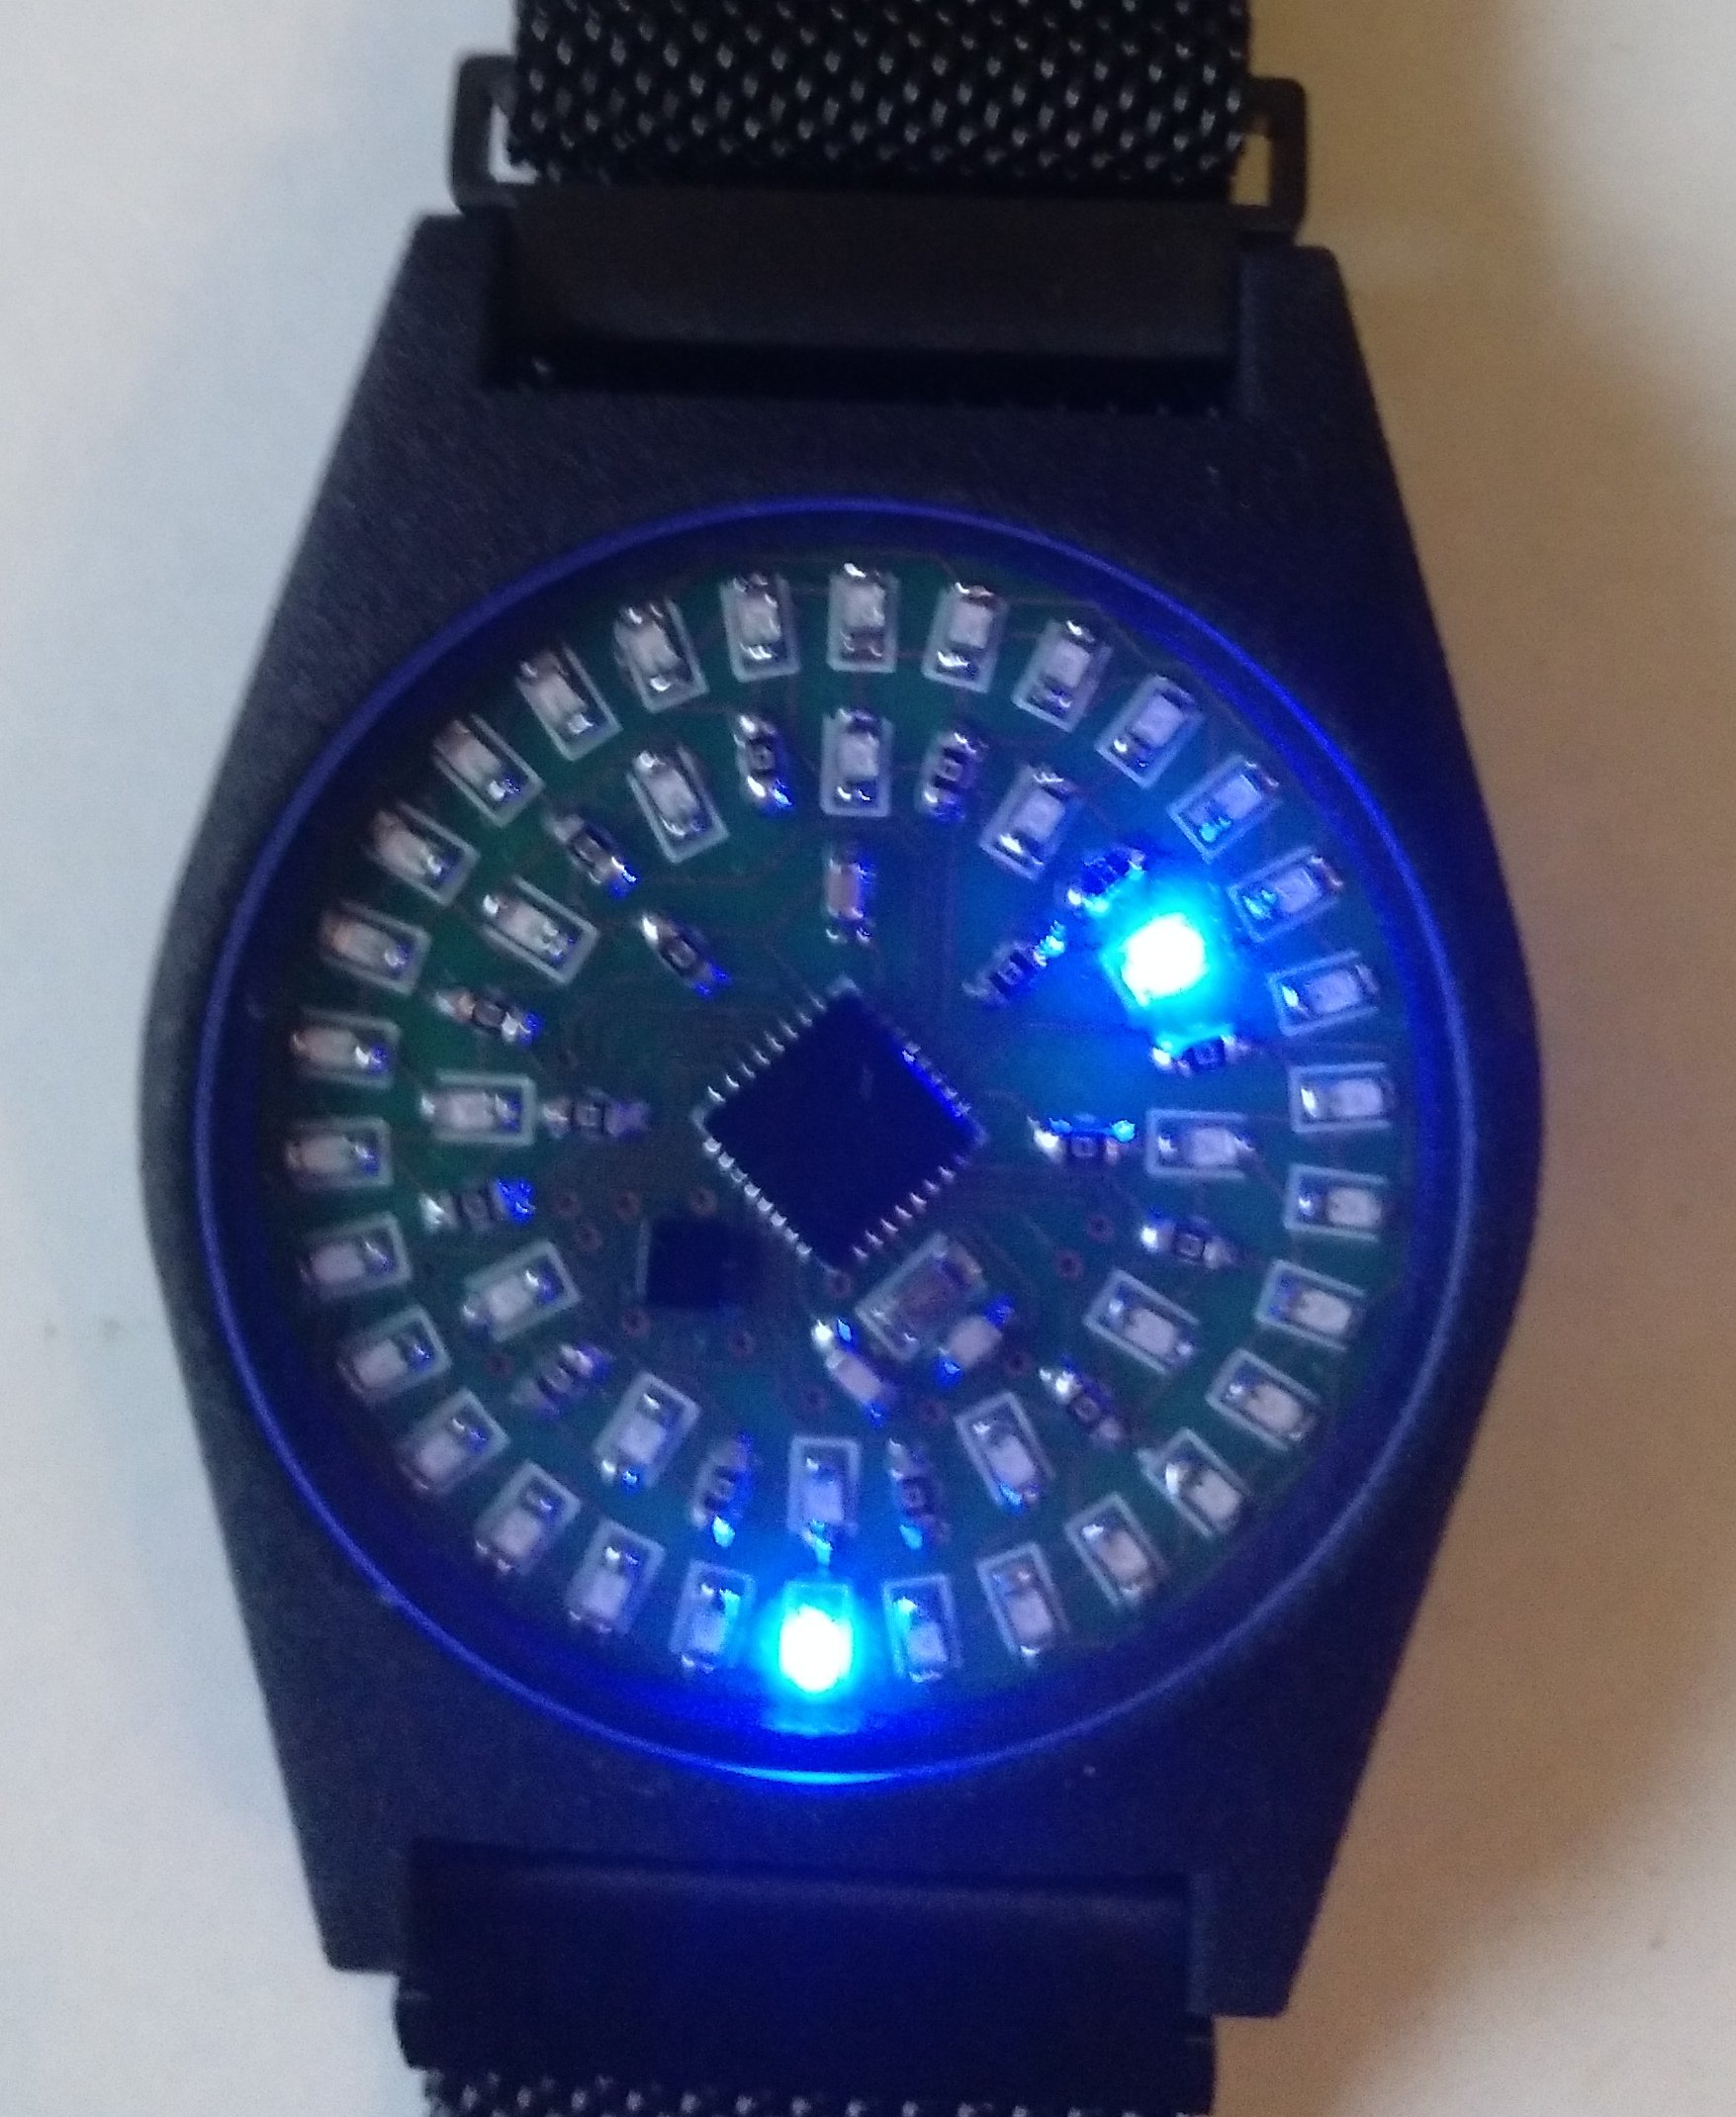
\includegraphics[width=0.45\textwidth]{../Pictures/AnalogSTM.jpg}
\end{center}

\paragraph{Software for the Analog Version}
I wanted to keep the changes on the Software as simple as possible and don't want to maintain two folders with common files between both variants. I created a combined software, which selects the correct \verb!DisplayManager! depending on  the watch variant saved in the flash, right next to the calibration values for the RTC. So i have only one Software, which fits the analog and the binary version of the watch, but i need to specify, via a define in the calibration software, if it is a analog or a binary watch. For further development i also added some defines in the software, which can disable a specific watch variant. This can be used either to save flash memory or to reduce the possible software bugs in the software.


\end{document}